
\documentclass[letterpaper]{article}

\usepackage{graphicx}
\usepackage{url}
\usepackage{float}


\title{Does the Version Control System affect commit understandability?}
\author{Mihai Codoban \and Caius Brindescu}
\date{}

\begin{document}

\maketitle

\section{Research questions}

\begin{enumerate}
	\item Do SVN commits take more time to understand than Git commits?
	\item Does user background (programming experience, industry experience etc) influence the time it takes to understand a commit?
	\item Does user background influence the quality and depth of the understanding of a commit or change description?
	\item Is there a common leave of change description between people?
\end{enumerate}

\section{Method}

\subsection{Participants}

Our participants are Java developers with Version Control Systems (VCS) experience. 
This includes:
\begin{itemize}
	\item at least 5 years of programming experience
	\item at least 1 year of experience using Java
	\item at least 1 year of experience using a VCS
\end{itemize}

Participants are recruited via email lists, university announcements (electronic and billboards), and local software companies targeting.

We will have 30 participants (5 people x 6 sessions). 
We plan on recruiting 47 people (30 participants, 2 no-shows per session and 5 pilots).

\subsection{Apparatus or Materials}

Participants will be viewing commits in a custom made software that for each commit shows the commit message, the diff (using the Eclipse Comparator Editor) and a text box where the commit description would be written.
They will have the following materials:
\begin{itemize}
	\item checklist of items to look for when understanding commits (embedded in commit window)
	\item commit information (commit message and commit diffs)
	\item questionnaire
\end {itemize}

Each participant described 3 SVN commits and 3 Git commits.
Each commit is chosen from a different repository.
Repositories are chosen from the top 6 Java repositories.
We selected 3 repositories using Git from GitHub and 3 repositories using SVN from SourceForge.
A commit is randomly chosen from the last commits in a project.
We believe this the last commits are representative of the change done in the later stages of the development.
To ensure the integrity of the commits we ignore commits that 
\begin{itemize}
	\item Contain changes to non-Java source files (build scripts, configuration files, etc);
	\item Are merge commits (this applies for Git only);
	\item Only change the formatting or comments.
\end{itemize}

\subsection{Procedure}

This will be a within subjects study. 
Each participant has to understand and describe 3 SVN commits and 3 Git commits. 
Their order in which we will apply the treatments will be random for each participant. 
This is done to eliminate the learning effect. 
The order will be determined by throwing a 6-sided die (or its programmatic equivalent).

The following script will be followed for each session:
\begin{enumerate}
	\item Informed Consent
	\item Administer tutorial
	\begin{enumerate}
		\item Explain the UI
		\item Explain the tasks to the participants
		\item Do a demo task
		\item Do a practice task
	\end{enumerate}
	\item Practice Task
	\item Tasks
	\begin{enumerate}
		\item Each task contains the commit message and the commit changes.
		\item The participant has to understand the commit. We provide a checklist of items to check.
		\item The participants are instructed to maximize detail
	\end{enumerate}
	\item Administer post session questionnaire
	\item Pay participants and receive receipts 
\end{enumerate}

\section{Data}

For each participant, we will collect the following:
\begin{enumerate}
	\item Time when they start a task
	\item Time when they complete a task
	\item The description of the commit
	\item Timestamp of all the key presses.
	\item Post-session questionnaire
\end{enumerate}

The time needed to understand a commit is determined by subtracting from the time it took to complete a task, the time it took the participants to type in their answer.
This will eliminate any variation due to varying typing speeds.
This variation can be seen in figure \ref{fig:typingTimes}.

\begin{figure}[H]
    \centering
    \includegraphics[width=0.7\textwidth]{../data/analysis/typingTime.pdf}
    \caption{Variation between participant typing times. The time for each participant is computed by averaging all the participant's task times.}
    \label{fig:typingTimes}
\end{figure}

\section{Results}

\subsection{RQ1: Is the commit understanding time influenced by the VCS?}

%how data looks
To answer this research question we looked at how long it took participants to understand commits.
Each participant produced 6 understand times, 3 for SVN and 3 for Git.
For each participant we averaged the SVN times and Git times thus obtaining two times for the two VCS tools.
We then separated these times in two bins: one bin of SVN times and one bin of Git times. 
The averaging of times per participant was done so as not to have related data (more times from the same participant) in the same bin.
Figure \ref{fig:rq1-data} shows how we arranged the data.

\begin{figure}[H]
    \centering
    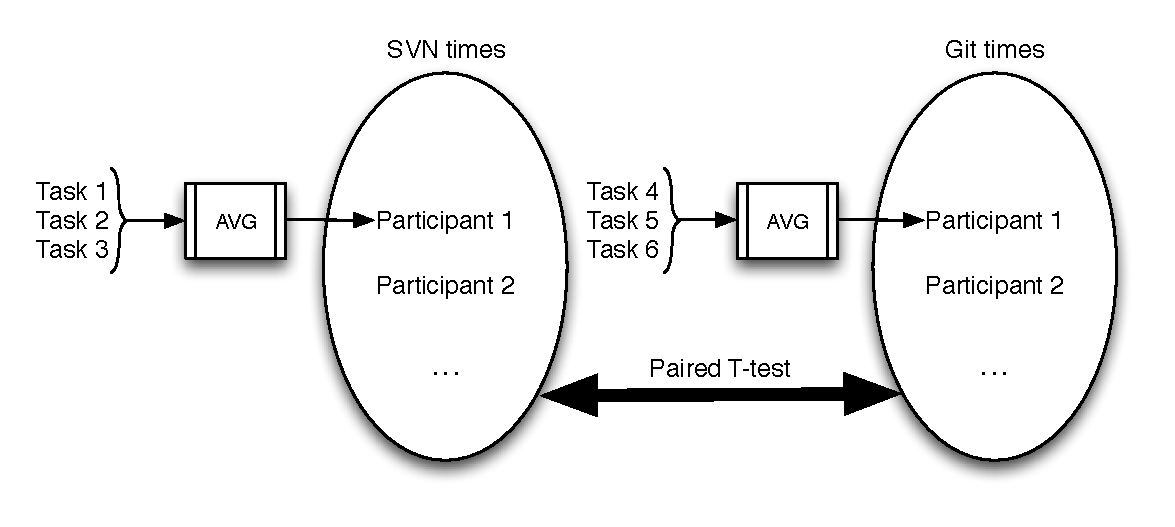
\includegraphics[width=1\textwidth]{fig/RQ1-data}
    \caption{RQ1 data aggregation. Task 1, 2 and 3 represent the SVN tasks whereas Task 4, 5 and 6 represent the Git tasks.}
    \label{fig:rq1-data}
\end{figure}

%what test we used on this data
To test whether the SVN times are different from the Git we performed a paired T-test.
The test is paired because one SVN data point is connected to one Git data point by the fact that they come from the same participant.
We thus tested whether participants require different times to understand commits under different VCS tools.

%results of test
The participants took a longer time to understand SVN commits than Git commits (t = 11.535, df = 29, p-value = 2.352e-12). The difference between the means of the two groups is 2.23 minutes.

%show plots and describe data 
Figure \ref{fig:rq1-understandTimes} shows the distribution of the overall commit understand times (Git + SVN).


%interpretation

\subsection{RQ2: Does the user background (programming experience, etc) influence the time it takes to understand a commit?}

\subsection{RQ3: Does the user background influence the quality and the depth of understanding a commit or a change description?}

\subsection{RQ4: Is there a common level of change description between people?}

\section{Discussion}

\subsection{Threats to validity}

\subsubsection{Internal Threats}

\paragraph{Maturation.}
The participants had to describe a total of 6 commits.
Some participants complained that this activity was hard and boring.
Therefore there is the risk that participants' effort of understanding decreased with time.
We mitigate this risk by randomizing the order in which each participant received the tasks.

\subsubsection{External Threats}

\paragraph{Commit Selection.}
While the commits were selected randomly, there is a possibility that they are not representative for the general practice.
Projects have thousands of commits and we randomly chose one from each project.
We tried to pick typical code change commits by choosing from the last commit in a project and filtering noisy commits.

\paragraph{Tool.}
For this study we build a special tool. 
This might be different than the tools used in the wild.
However, for representing the commits we chose the standard Eclipse commit viewer.
This is a well known graphical model of viewing commits.

\paragraph{Selection.}
In terms of the population, our results are representative of experienced programmers an experiences VCS users.
We do not know how the lack of experience might impact commit u

\subsubsection{Construct Threats}

\paragraph{Personal bias of understanding.}
The participants had to self-assess when they understood all the changes. 
This varies from person to person. 
Offering a checklist and grading the responses tried to mitigate this risk as much as possible.

\paragraph{Measuring understanding.}
We measured the understanding time by subtracting the typing time from the total task time.
This subtraction is due to different typing times for different people.
However, except the typing time, participants may not have been mentally engaged in the task at all times.

\paragraph{Ambiguous survey question.}
The survey question involving VCS use and preference was reported as being ambiguous.
Participants were not sure whether to respond with their latest preferences or with their overall experience.

\subsubsection{Reliability Threats}

The details described in this paper are sufficient to recreate the experiment.
Moreover the source code of the tool, collected data, analysis scripts and the survey are publicly available\footnote{\url{github.com/cdmihai/CS589}} \footnote{http://goo.gl/uZM5vL}.

\end{document}